\chapter{Cơ sở lý thuyết và công nghệ}
\label{chap:co_so_ly_thuyet}

Chương này khảo sát các công trình liên quan (Mục~\ref{sec:c2_lien_quan}), trình bày nền tảng lý thuyết mà hệ thống dựa vào (Mục~\ref{sec:c2_ly_thuyet}) và các công nghệ sử dụng (Mục~\ref{sec:c2_cong_nghe}).

\section{Khảo sát các công trình liên quan}
\label{sec:c2_lien_quan}

\subsection{Truy hồi và hỏi đáp văn bản pháp luật tiếng Việt}

\textbf{Các cuộc thi và bộ dữ liệu.} Zalo AI Challenge 2021 có nhánh Legal Text Retrieval \cite{zalo2021legal}: cho một câu hỏi pháp luật tiếng Việt, hệ thống phải tìm các điều luật liên quan trong một kho văn bản. Ban tổ chức không công bố bài báo mô tả dữ liệu; bản được dùng nhiều là bản đưa lên Hugging Face và vào MTEB với tên ``ZacLegalTextRetrieval'' \cite{greennode_zalolegal} (kho khoảng 61 nghìn đoạn, phần câu hỏi 818 dòng). Cuộc thi ALQAC tổ chức cùng hội nghị KSE: ALQAC 2021 \cite{nguyen2021alqac} có ba nhiệm vụ là tìm điều luật, suy diễn pháp lý và hỏi đáp trên luật Việt Nam và Thái Lan; ALQAC 2022 \cite{nguyen2022alqac} và ALQAC 2023 \cite{nguyen2023alqac} giữ hai nhiệm vụ tìm văn bản và hỏi đáp trên luật Việt Nam.

Các bộ dữ liệu mới hơn mở rộng sang hỏi đáp và suy luận. VLQA \cite{nguyen2025vlqa} là bộ dữ liệu hỏi đáp pháp luật tiếng Việt dùng để đánh giá cả tìm kiếm và hỏi đáp. VLegal-Bench \cite{dong2025vlegalbench} có 10.450 mẫu tổ chức theo các mức nhận thức, gồm hỏi đáp, RAG, suy luận nhiều bước và giải tình huống. ViBidLQA \cite{nguyen2024vibidlqa} là bộ hỏi đáp luật đấu thầu do mô hình ngôn ngữ sinh rồi chuyên gia sửa lại, dùng để so sánh hướng trích đoạn (MRC) với hướng sinh câu trả lời. Gần lĩnh vực của đề tài nhất là VLSP 2025 MLQA-TSR \cite{luu2025vlsp}, hỏi đáp đa phương thức về quy định biển báo giao thông đường bộ Việt Nam, với kết quả tốt nhất F2 = 64,55\% cho nhiệm vụ tìm điều luật và độ chính xác 86,30\% cho nhiệm vụ trả lời.

\textbf{Các phương pháp.} Pham và cộng sự \cite{pham2022multistage} dùng sentence-transformers trên nền PhoBERT \cite{nguyen2020phobert} và so sánh nhiều cách kết hợp điểm BM25 với điểm cosine; trên một kho khoảng 114 nghìn điều luật, cấu hình tốt nhất đạt F2 = 0,741. Nguyen và cộng sự \cite{nguyen2024attentive} đề xuất các mạng chú ý phân cấp (Attentive CNN, Paraformer) cho tìm văn bản pháp luật đa ngôn ngữ. Nhóm BKAI \cite{duc2024bkai} huấn luyện một bi-encoder trên nền PhoBERT-base-v2, đạt Acc@1 = 73,28 và MRR@10 = 80,73 trên phần kiểm tra của Zalo 2021 theo trang mô tả mô hình. Pham Tien và cộng sự \cite{pham2024synthetic} tiền huấn luyện bi-encoder và ColBERT trên câu hỏi do mô hình ngôn ngữ lớn sinh ra. Nguyen Ba và cộng sự \cite{nguyenba2024legalir} mô tả một hệ thống hỏi đáp gộp tìm theo từ khoá và theo vector bằng một biến thể của RRF rồi xếp hạng lại bằng mô hình ngôn ngữ lớn; về cách làm, đây là công trình gần thiết kế tìm lai của đề tài nhất. Phần lớn các công trình trên tách từ trước khi mã hoá bằng VnCoreNLP \cite{vu2018vncorenlp} hoặc pyvi \cite{tran_pyvi}.

\subsection{Sinh câu trả lời có tăng cường truy xuất và agent}

Lewis và cộng sự \cite{lewis2020rag} đặt tên cho mô hình RAG: một mô hình sinh được ghép với bộ tìm kiếm vector DPR \cite{karpukhin2020dpr} trên Wikipedia, sao cho tri thức nằm một phần trong tham số mô hình và một phần trong chỉ mục ngoài có thể thay thế. Gao và cộng sự \cite{gao2023ragsurvey} phân loại các hướng RAG thành ba dạng: \emph{Naive RAG} tìm một lần rồi sinh; \emph{Advanced RAG} thêm xử lý trước và sau khi tìm như viết lại câu hỏi và xếp hạng lại; \emph{Modular RAG} ghép các thành phần linh hoạt và có thể lặp. Về đơn vị tìm kiếm, Jimeno Yepes và cộng sự \cite{jimeno2024chunking} cắt văn bản theo loại phần tử thay vì theo độ dài cố định; Chen và cộng sự \cite{chen2023densex} cho thấy đơn vị mịn hơn (mệnh đề) tốt hơn đơn vị đoạn văn; Anthropic \cite{anthropic2024contextual} đề xuất ghép ngữ cảnh vào trước mỗi đoạn trước khi lập chỉ mục, và báo cáo tỉ lệ trượt giảm từ 5,7\% xuống 2,9\% khi thêm ngữ cảnh cho cả vector và BM25. Trong miền pháp lý tiếng Anh, LegalBench-RAG \cite{pipitone2024legalbenchrag} là bộ đánh giá riêng cho bước tìm kiếm của RAG với 6.858 cặp câu hỏi--đáp án.

ReAct \cite{yao2023react} cho mô hình ngôn ngữ xen kẽ bước suy luận với bước hành động như gọi API tìm kiếm, rồi đọc kết quả để quyết định bước sau. Toolformer \cite{schick2023toolformer} huấn luyện mô hình tự quyết định khi nào gọi API. IRCoT \cite{trivedi2023ircot} dùng từng bước của chuỗi suy luận làm truy vấn cho lần tìm tiếp theo và tăng tới 21 điểm về tìm kiếm trên các bộ câu hỏi nhiều bước. Self-RAG \cite{asai2024selfrag} huấn luyện mô hình tự quyết định khi nào cần tìm và tự chấm câu trả lời. Singh và cộng sự \cite{singh2025agentic} tổng hợp các hệ thống RAG dạng agent theo số agent, cấu trúc điều khiển và mức tự chủ. Model Context Protocol \cite{anthropic2024mcp} là giao thức mở chuẩn hoá cách ứng dụng mô hình ngôn ngữ kết nối với nguồn dữ liệu và công cụ.

\subsection{So sánh với hệ thống của đề tài}

Bảng~\ref{tab:c2_so_sanh} so sánh các công trình tiêu biểu với hệ thống của đề tài theo miền dữ liệu, đơn vị truy hồi, việc xét hiệu lực theo thời gian và cách tìm kiếm, sinh câu trả lời.

\begin{table}[htbp]
\centering
\caption{So sánh các công trình liên quan với hệ thống của đề tài}
\label{tab:c2_so_sanh}
\footnotesize
\renewcommand{\arraystretch}{1.05}
\begin{tabularx}{\textwidth}{@{}>{\raggedright\arraybackslash}p{2.6cm} >{\raggedright\arraybackslash}X >{\raggedright\arraybackslash}p{1.7cm} >{\raggedright\arraybackslash}p{1.5cm} >{\raggedright\arraybackslash}X@{}}
\toprule
\textbf{Công trình} & \textbf{Miền và nhiệm vụ} & \textbf{Đơn vị} & \textbf{Xét hiệu lực} & \textbf{Tìm kiếm / sinh} \\
\midrule
Zalo 2021 \cite{zalo2021legal} & Luật Việt Nam; tìm điều luật & Điều & Không & Bộ dữ liệu chuẩn \\
ALQAC \cite{nguyen2021alqac,nguyen2023alqac} & Luật Việt Nam; tìm điều luật, hỏi đáp & Điều & Không & Bộ dữ liệu chuẩn \\
ViBidLQA \cite{nguyen2024vibidlqa} & Luật đấu thầu; hỏi đáp & -- & Không & So sánh MRC và sinh \\
VLSP 2025 \cite{luu2025vlsp} & Biển báo giao thông; đa phương thức & Điều & Không & Chữ và ảnh \\
Pham và cs. \cite{pham2022multistage} & Luật Việt Nam; tìm điều luật & Điều & Không & PhoBERT kết hợp BM25 \\
Nguyen Ba và cs. \cite{nguyenba2024legalir} & Luật Việt Nam; hỏi đáp & -- & Không & Biến thể RRF, xếp hạng lại bằng LLM \\
RAG \cite{lewis2020rag} & Wikipedia; hỏi đáp miền mở & Đoạn Wikipedia & Không & DPR, sinh một lần \\
ReAct \cite{yao2023react} & Hỏi đáp, ra quyết định & Kết quả tìm Wikipedia & Không & Agent gọi API tìm kiếm \\
\midrule
\textbf{Đề tài} & Luật giao thông đường bộ Việt Nam; tra cứu và hỏi đáp & Điểm & Có, theo ngày vi phạm và ghi chú sửa đổi & Vector + BM25 (RRF) + nguyên văn; agent nhiều bước qua MCP \\
\bottomrule
\end{tabularx}
\end{table}

So với các công trình trên, đề tài khác ở bốn điểm. Thứ nhất, đơn vị tìm kiếm là Điểm thay vì cả Điều, vì mức phạt và hành vi nằm ở hai cấp khác nhau của nghị định xử phạt. Thứ hai, kho văn bản không tĩnh: kết quả được lọc theo ngày vi phạm và gắn ghi chú văn bản sửa đổi. Thứ ba, bộ đánh giá câu trả lời được soạn theo lời hỏi thật, có câu không dấu và viết tắt, và nhánh BM25 dùng âm tiết, cặp âm tiết không dấu thay cho bước tách từ. Thứ tư, cần nêu rõ một hạn chế: hệ thống chưa được chạy trên Zalo 2021 hay ALQAC và chưa so với bi-encoder BKAI \cite{duc2024bkai}, nên các con số của đề tài không so trực tiếp được với các con số của những công trình này.

\section{Nền tảng lý thuyết}
\label{sec:c2_ly_thuyet}

\subsection{Văn bản quy phạm pháp luật và cấu trúc phân cấp}
\label{subsec:c2_vbqppl}

Văn bản quy phạm pháp luật Việt Nam được sắp theo thứ bậc của cơ quan ban hành: luật của Quốc hội quy định nguyên tắc chung; nghị định của Chính phủ quy định chi tiết và xử phạt; thông tư của Bộ trưởng hướng dẫn nội dung kỹ thuật và thủ tục; quy chuẩn kỹ thuật quốc gia ban hành kèm theo thông tư. Luật được sửa đổi nhiều lần có văn bản hợp nhất ghép nội dung gốc với nội dung sửa đổi; ba luật trong kho được nạp ở dạng này (Bảng~\ref{tab:c1_kho_van_ban}). Theo quy ước soạn thảo, nội dung một văn bản được chia thành các cấp lồng nhau: Phần, Chương, Mục, Tiểu mục, Điều, Khoản, Điểm. Mỗi cấp có cách đánh số riêng: Chương đánh số La Mã (``Chương II''), Điều đánh số Ả Rập kèm tiêu đề (``Điều 6.''), Khoản đánh số Ả Rập có dấu chấm (``1.''), Điểm đánh chữ cái tiếng Việt có ngoặc đơn (``a)'', ``đ)''). Khi văn bản được sửa đổi, các cấp chèn thêm mang hậu tố như \texttt{12a}, \texttt{IIa}, \texttt{a1}. Hình~\ref{fig:c2_cay_van_ban} minh hoạ cây phân cấp với một đường đi cụ thể trong Nghị định 168/2024/NĐ-CP.

\begin{figure}[htbp]
\centering
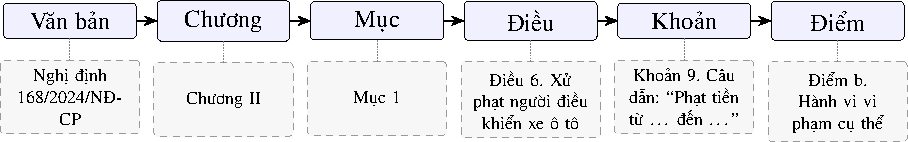
\includegraphics{graphics/fig_ch2_1.pdf}
\caption{Cấu trúc phân cấp của văn bản quy phạm pháp luật và một ví dụ trong nghị định xử phạt}
\label{fig:c2_cay_van_ban}
\end{figure}

Hai quy ước có ý nghĩa đặc biệt với việc truy hồi. Thứ nhất, trong nghị định xử phạt, mức tiền nằm ở câu dẫn của Khoản, còn hành vi nằm ở các Điểm bên dưới, nên một Điểm đứng riêng không trả lời được câu hỏi ``phạt bao nhiêu''. Thứ hai, văn bản sửa đổi chép lời văn mới trong ngoặc kép (``a) Sửa đổi, bổ sung điểm đ như sau:'' rồi tới dòng ``đ)'' trong ngoặc kép); nếu không xử lý ngoặc kép, dòng này bị hiểu nhầm thành một Điểm của chính văn bản sửa đổi. Văn bản cũng tự trích dẫn nội bộ theo khuôn mẫu ổn định như ``điểm a khoản 9 Điều này'' hay ``Điều 5 Thông tư này'', cho phép giải liên kết trích dẫn tất định trên cây đã phân tích.

\subsection{Mô hình BM25}
\label{subsec:c2_bm25}

BM25 là hàm xếp hạng thuộc khung xác suất về mức liên quan \cite{robertson2009bm25}, kết hợp trọng số nghịch đảo tần suất văn bản (IDF), theo đó từ hiếm quan trọng hơn từ phổ biến, tần suất từ có bão hoà (tham số $k_1$) và chuẩn hoá theo độ dài (tham số $b$). Với kho gồm $N$ đoạn, $n_t$ là số đoạn chứa từ $t$, IDF và điểm BM25 của đoạn $d$ đối với truy vấn $q$ là:
\begin{equation}
\label{eq:c2_idf}
\mathrm{IDF}(t) = \ln\left(1 + \frac{N - n_t + 0{,}5}{n_t + 0{,}5}\right).
\end{equation}
\begin{equation}
\label{eq:c2_bm25}
\mathrm{BM25}(q, d) = \sum_{t \in q} \mathrm{IDF}(t) \cdot \frac{\mathrm{tf}(t, d)\,(k_1 + 1)}{\mathrm{tf}(t, d) + k_1 \left(1 - b + b\,\dfrac{|d|}{\mathrm{avgdl}}\right)},
\end{equation}
trong đó $\mathrm{tf}(t, d)$ là số lần từ $t$ xuất hiện trong $d$, $|d|$ là độ dài của $d$ và $\mathrm{avgdl}$ là độ dài trung bình của các đoạn. Hệ thống dùng các giá trị thông dụng $k_1 = 1{,}2$ và $b = 0{,}75$, không chỉnh theo bộ đề. Khi $\mathrm{tf}(t,d)$ tăng, phân số trong~\eqref{eq:c2_bm25} tiến dần về $k_1 + 1$ thay vì tăng tuyến tính, nên một từ lặp nhiều lần không lấn át các từ khác; khi $|d| > \mathrm{avgdl}$, điểm giảm, nên đoạn dài không được lợi chỉ vì chứa nhiều chữ. Hàm \texttt{ts\_rank} có sẵn của PostgreSQL không có hai tính chất này: nó không có IDF, nên các từ có mặt ở hầu hết các đoạn như ``xe'' hay ``giao thông'' nặng ngang từ hiếm, và nó không chuẩn hoá độ dài.

Đề tài áp dụng BM25 cho tiếng Việt mà không tách từ: văn bản được bỏ dấu, chuyển chữ thường và tách thành âm tiết; mỗi đoạn sinh ra âm tiết đơn và cặp hai âm tiết liền nhau (``đèn tín hiệu'' sinh \texttt{den\_tin} và \texttt{tin\_hieu}, đủ để phân biệt với ``tín hiệu'' đứng riêng mà không cần từ điển). Vì cả kho và câu hỏi đều bỏ dấu trước khi tách, câu gõ không dấu vẫn khớp được với văn bản có dấu.

\subsection{Tìm kiếm theo vector và độ tương tự cosine}
\label{subsec:c2_dense}

Tìm kiếm theo vector (dense retrieval) mã hoá câu hỏi và đoạn văn thành vector trong cùng một không gian, sao cho các cặp liên quan nằm gần nhau. DPR \cite{karpukhin2020dpr} dùng hai bộ mã hoá BERT huấn luyện bằng học tương phản và vượt BM25 từ 9 đến 19 điểm phần trăm về độ chính xác top-20 trên các bộ hỏi đáp miền mở. Tuy vậy, đánh giá BEIR \cite{thakur2021beir} trên 18 bộ dữ liệu cho thấy BM25 là một mốc so sánh vững và nhiều mô hình vector tụt điểm khi chuyển sang miền mới.

Mức gần nhau giữa vector câu hỏi $\mathbf{q}$ và vector đoạn $\mathbf{d}$ được đo bằng độ tương tự cosine:
\begin{equation}
\label{eq:c2_cosine}
\cos(\mathbf{q}, \mathbf{d}) = \frac{\mathbf{q} \cdot \mathbf{d}}{\lVert \mathbf{q} \rVert \, \lVert \mathbf{d} \rVert}.
\end{equation}
Khi mọi vector đã được chuẩn hoá L2, cosine bằng tích vô hướng và khoảng cách cosine bằng $1 - \cos(\mathbf{q}, \mathbf{d})$. Để không phải so câu hỏi với mọi đoạn, cơ sở dữ liệu dùng chỉ mục HNSW, một đồ thị lân cận nhiều tầng cho phép tìm lân cận gần đúng nhanh.

Theo Matryoshka Representation Learning \cite{kusupati2022mrl}, mô hình được huấn luyện sao cho các tiền tố của vector embedding cũng là biểu diễn dùng được, nên có thể cắt bớt chiều mà mất ít chất lượng. Với vector gốc $\mathbf{v} \in \mathbb{R}^{1024}$, hệ thống giữ 512 chiều đầu và chuẩn hoá lại:
\begin{equation}
\label{eq:c2_mrl}
\tilde{\mathbf{v}} = \frac{(v_1, v_2, \ldots, v_{512})}{\lVert (v_1, v_2, \ldots, v_{512}) \rVert_2}.
\end{equation}
Cắt còn một nửa số chiều giúp giảm một nửa dung lượng lưu trữ và chi phí tính khoảng cách.

\subsection{Reciprocal Rank Fusion}
\label{subsec:c2_rrf}

Tìm kiếm lai kết hợp danh sách xếp hạng của nhánh vector và nhánh BM25; hai nhánh có thang điểm khác nhau nên không cộng điểm trực tiếp được. Reciprocal Rank Fusion \cite{cormack2009rrf} chỉ dùng thứ hạng:
\begin{equation}
\label{eq:c2_rrf}
\mathrm{RRF}(d) = \sum_{r \in R} \frac{1}{k + r(d)},
\end{equation}
trong đó $R$ là tập các danh sách xếp hạng, $r(d)$ là hạng của $d$ trong danh sách $r$ (bắt đầu từ 1), và $d$ không có trong một danh sách thì không nhận số hạng tương ứng. Bài báo gốc dùng $k = 60$, giá trị được cố định trong một khảo sát thử nghiệm ban đầu chứ không suy ra từ lý thuyết; Bruch và cộng sự \cite{bruch2023fusion} cho thấy RRF nhạy với tham số này và tổ hợp lồi của các điểm đã chuẩn hoá có thể tốt hơn. Hằng số $k$ điều khiển mức chênh lệch giữa các hạng đầu. Với $k = 60$, hạng 1 nhận $1/61 \approx 0{,}0164$ còn hạng 10 nhận $1/70 \approx 0{,}0143$, nên một kết quả đứng đầu ở một nhánh nhưng vắng ở nhánh kia có thể bị một kết quả đứng thứ mười ở cả hai nhánh vượt qua. Đề tài dùng $k = 20$: hạng 1 nhận $1/21 \approx 0{,}0476$, gấp khoảng 1,6 lần hạng 10 ($1/30 \approx 0{,}0333$), giúp giữ lại các kết quả rất tốt của từng nhánh. Giá trị này được chọn bằng cách quan sát tập dev, và khác biệt so với $k = 60$ trên tập dev chỉ là 4 câu.

\subsection{Mô hình embedding Qwen3-Embedding}
\label{subsec:c2_qwen3}

Qwen3 Embedding \cite{zhang2025qwen3} là họ mô hình embedding và xếp hạng lại dựng trên mô hình nền Qwen3, hỗ trợ chọn số chiều đầu ra theo kiểu Matryoshka và nhận chỉ dẫn cho câu hỏi. Theo báo cáo kỹ thuật, cả ba cỡ đều nhận tối đa 32K token; bản 0.6B có 1024 chiều và đạt 64,33 điểm MMTEB \cite{enevoldsen2025mmteb} (trung bình theo nhiệm vụ), bản 4B có 2560 chiều và đạt 69,45, bản 8B có 4096 chiều và đạt 70,58; trong cùng bảng so sánh, multilingual-e5-large-instruct \cite{wang2024me5} đạt 63,22 và BGE-M3 \cite{chen2024m3} đạt 59,56.

Hệ thống dùng Qwen3-Embedding-0.6B, cắt từ 1024 xuống 512 chiều theo công thức~\eqref{eq:c2_mrl}. Câu hỏi được mã hoá kèm prompt truy vấn của mô hình, một dòng chỉ dẫn đứng trước câu hỏi (\texttt{Instruct: \ldots{} Query: \ldots}); các đoạn văn bản được mã hoá không kèm prompt. Bản 0.6B được chọn vì lý do thực dụng: đa ngôn ngữ, nhận chuỗi dài và chạy được trên GPU 4 GB của máy phát triển. Bản 4B cần khoảng 8 GB trọng số ở fp16 nên chưa được đo trên kho hiện tại. Các bộ đánh giá MTEB \cite{muennighoff2023mteb} và MMTEB \cite{enevoldsen2025mmteb} đều cho thấy không có mô hình nào thắng ở mọi nhiệm vụ, nên việc đo trực tiếp trên dữ liệu của bài toán là cần thiết.

\subsection{Agent dựa trên mô hình ngôn ngữ lớn và giao thức MCP}
\label{subsec:c2_agent_mcp}

Trong Naive RAG \cite{gao2023ragsurvey}, câu hỏi được dùng trực tiếp làm truy vấn và mô hình sinh câu trả lời trong một lượt. Cách này nhanh nhưng phụ thuộc hoàn toàn vào lần tìm duy nhất: nếu câu khẩu ngữ khiến bộ tìm kiếm lệch chủ đề, mô hình không có cách nào sửa. Agent theo kiểu ReAct \cite{yao2023react} dùng một vòng lặp: suy luận về bước cần làm, gọi công cụ, đọc kết quả, rồi quyết định tìm lại, đọc rộng ra hay trả lời (Hình~\ref{fig:c2_rag_agent}).

\begin{figure}[htbp]
\centering
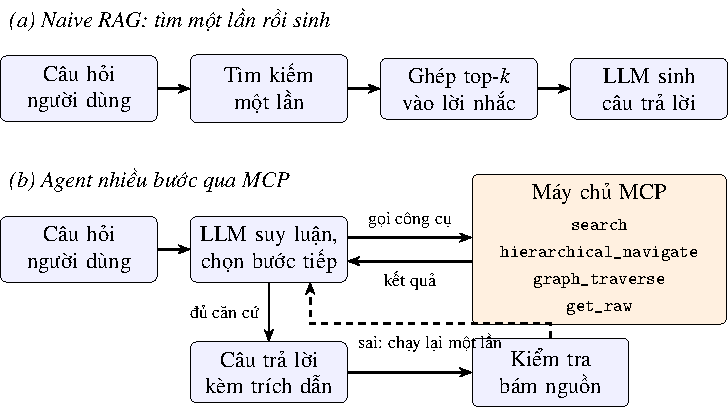
\includegraphics{graphics/fig_ch2_2.pdf}
\caption{So sánh luồng RAG tìm một lần với vòng lặp agent gọi công cụ qua MCP}
\label{fig:c2_rag_agent}
\end{figure}

Một agent cần một mô hình ngôn ngữ có khả năng gọi hàm, một tập công cụ được mô tả bằng tên, tham số và chú thích, và một vòng điều khiển giới hạn số lượt và thời gian. Khác với Toolformer \cite{schick2023toolformer} hay Self-RAG \cite{asai2024selfrag}, đề tài không huấn luyện thêm mô hình nào; hành vi của agent được điều khiển bằng lời nhắc và mô tả công cụ, nên đóng góp nằm ở thiết kế công cụ cho miền pháp luật chứ không ở cơ chế agent.

MCP \cite{anthropic2024mcp} là giao thức mở do Anthropic công bố tháng 11/2024, chuẩn hoá cách một ứng dụng dùng mô hình ngôn ngữ (client) kết nối với nguồn dữ liệu và công cụ (server): máy chủ khai báo công cụ với tên, mô tả và lược đồ tham số; client đưa mô tả cho mô hình và chuyển lời gọi do mô hình sinh ra tới máy chủ, nên cùng một máy chủ phục vụ được nhiều client mà không phải viết lại phần tích hợp. Trong đề tài, máy chủ MCP cung cấp bốn công cụ chỉ đọc \texttt{search}, \texttt{hierarchical\_navigate}, \texttt{graph\_traverse} và \texttt{get\_raw}; client là Claude Code chạy ở chế độ không tương tác, chỉ được gọi bốn công cụ này, tối đa 10 lượt và 300 giây cho mỗi câu hỏi; công cụ có khả năng ghi vào đồ thị trích dẫn nằm ngoài danh sách được phép.

\subsection{Các độ đo đánh giá}
\label{subsec:c2_do_do}

\textbf{Hit@k và MRR.} Gọi $Q$ là tập câu hỏi và $\mathrm{rank}_q$ là hạng của điều khoản đáp án đầu tiên trong kết quả cho câu hỏi $q$ (bằng $\infty$ nếu không tìm thấy, quy ước $1/\infty = 0$); một kết quả được coi là trúng khi nó là điều khoản đáp án hoặc nằm dưới điều khoản đáp án trong cây. Hit@k là tỉ lệ câu có đáp án trong $k$ kết quả đầu, còn Mean Reciprocal Rank là trung bình nghịch đảo hạng của đáp án:
\begin{equation}
\label{eq:c2_mrr}
\mathrm{Hit@}k = \frac{1}{|Q|} \sum_{q \in Q} \mathbf{1}\left[\mathrm{rank}_q \le k\right], \qquad
\mathrm{MRR} = \frac{1}{|Q|} \sum_{q \in Q} \frac{1}{\mathrm{rank}_q}.
\end{equation}
Hit@1 đo khả năng đưa đáp án lên đầu, Hit@k với $k$ lớn đo độ phủ, còn MRR thưởng cho việc đưa đáp án lên càng cao càng tốt.

\textbf{Kiểm định McNemar.} Khi so hai cấu hình A và B trên cùng một tập câu hỏi, các câu mà cả hai cùng đúng hoặc cùng sai không mang thông tin về khác biệt. Gọi $b$ là số câu A đúng mà B sai, $c$ là số câu A sai mà B đúng. Kiểm định McNemar \cite{mcnemar1947} kiểm tra giả thuyết không rằng hai loại bất đồng có cùng xác suất. Dạng chính xác dùng phân phối nhị thức với $n = b + c$:
\begin{equation}
\label{eq:c2_mcnemar}
p = \min\left(1,\; 2 \sum_{i=0}^{\min(b, c)} \binom{n}{i} \left(\frac{1}{2}\right)^{n}\right).
\end{equation}
Dạng chính xác phù hợp khi $b + c$ nhỏ, như khi hai cấu hình chỉ khác nhau ở vài câu (ví dụ đổi $k$ của RRF ở Mục~\ref{sec:ch5-tim-kiem}).

\textbf{Khoảng tin cậy Wilson.} Với tỉ lệ quan sát $\hat{p}$ trên $n$ mẫu, khoảng tin cậy Wilson ứng với giá trị tới hạn $z$ ($z = 1{,}96$ cho mức tin cậy 95\%) là:
\begin{equation}
\label{eq:c2_wilson}
\frac{\hat{p} + \dfrac{z^2}{2n} \pm z\sqrt{\dfrac{\hat{p}(1 - \hat{p})}{n} + \dfrac{z^2}{4n^2}}}{1 + \dfrac{z^2}{n}}.
\end{equation}
Khác với khoảng Wald $\hat{p} \pm z\sqrt{\hat{p}(1-\hat{p})/n}$, khoảng Wilson không vượt quá $[0, 1]$ và vẫn đáng tin khi $\hat{p}$ gần 0 hoặc 1 với mẫu nhỏ, đúng là tình huống của bộ đánh giá câu trả lời (Mục~\ref{sec:ch5-cau-tra-loi}).

\textbf{Đánh giá câu trả lời.} RAGAS \cite{es2024ragas} và ARES \cite{saadfalcon2024ares} dùng mô hình ngôn ngữ để chấm độ trung thành và độ liên quan; ALCE \cite{gao2023alce} đánh giá chất lượng trích dẫn. Đề tài chấm bằng quy tắc dựa trên đáp án tra tay (Mục~\ref{sec:ch5-cau-tra-loi}); tiêu chí ``mọi số Điều, số tiền trong câu trả lời đều có trong nguồn được trích'' là một dạng hẹp của độ trung thành và chất lượng trích dẫn, nhắm vào hai loại lỗi nguy hiểm nhất trong miền pháp luật mà \cite{magesh2025hallucination} đã chỉ ra: trích dẫn hoặc con số nghe hợp lý nhưng sai.

\section{Công nghệ sử dụng}
\label{sec:c2_cong_nghe}

Bảng~\ref{tab:c2_cong_nghe} liệt kê các công nghệ chính và vai trò của từng công nghệ trong hệ thống.

\begin{table}[htbp]
\centering
\caption{Các công nghệ sử dụng và vai trò trong hệ thống}
\label{tab:c2_cong_nghe}
\footnotesize
\renewcommand{\arraystretch}{1.05}
\begin{tabularx}{\textwidth}{@{}>{\raggedright\arraybackslash}p{4.6cm} >{\raggedright\arraybackslash}X@{}}
\toprule
\textbf{Công nghệ} & \textbf{Vai trò} \\
\midrule
Python $\geq$ 3.13, \texttt{uv} & Ngôn ngữ chính cho luồng nạp, bộ tìm kiếm, máy chủ MCP, API web và công cụ đánh giá, chạy bất đồng bộ trên \texttt{asyncio}; \texttt{uv} quản lý phụ thuộc (\texttt{uv.lock}) và chạy CLI \texttt{rag-eval} \\
PostgreSQL 16, \texttt{asyncpg} & Lưu văn bản, đoạn, chỉ mục ngược cho BM25, cạnh trích dẫn và bộ đệm vector; cài BM25 và tìm nguyên văn bằng hàm SQL; kết nối bất đồng bộ \\
\texttt{pgvector}, \texttt{ltree}, \texttt{unaccent} & Vector 512 chiều, tìm lân cận theo cosine với chỉ mục HNSW; đường dẫn phân cấp Chương--Điều--Khoản--Điểm, truy vấn theo nhánh cây; bỏ dấu \\
Docker Compose & Khởi chạy PostgreSQL kèm pgvector (container \texttt{pgvector/pgvector:pg16} trong \texttt{compose.yaml}) \\
\texttt{sentence-transformers}, \texttt{torch} & Chạy Qwen3-Embedding-0.6B để mã hoá câu hỏi và đoạn văn bản \\
\texttt{pdfplumber} & Nhánh trích xuất PDF (thử nghiệm) \\
FastAPI, \texttt{uvicorn}, Pydantic & API web cho hỏi đáp, tra cứu, danh mục văn bản và bộ đánh giá; kiểm tra dữ liệu vào ra \\
React 18, Vite, TypeScript, Tailwind CSS & Giao diện trang đơn gồm thẻ hỏi đáp, tra cứu điều luật và đánh giá tìm kiếm; song ngữ, ba chế độ màu \\
Claude Code CLI (\texttt{claude -p}) & Mô hình ngôn ngữ đóng vai trò agent, chạy không tương tác và gọi công cụ tra cứu qua MCP \\
Model Context Protocol (\texttt{mcp}) & Máy chủ MCP qua stdio, đưa bốn công cụ tra cứu chỉ đọc ra cho agent và các script đánh giá \\
\texttt{ruff}, \texttt{ty}, Playwright & Kiểm tra phong cách và kiểu tĩnh (\texttt{make check}); tự động hoá trình duyệt để kiểm thử giao diện \\
Git, GitHub & Quản lý mã nguồn, phát triển theo nhánh và pull request, lưu vết các thay đổi \\
\bottomrule
\end{tabularx}
\end{table}

Các công nghệ được chọn theo ba tiêu chí: mọi dữ liệu phục vụ tìm kiếm (văn bản, vector, chỉ mục từ khoá, đồ thị trích dẫn) nằm trong một cơ sở dữ liệu duy nhất, nên cả ba nhánh tìm kiếm cùng lọc theo ngày vi phạm và phạm vi văn bản trong một truy vấn SQL; mô hình embedding chạy cục bộ trên phần cứng phổ thông, không phụ thuộc dịch vụ ngoài khi tìm kiếm; và bộ công cụ tra cứu được tách khỏi mô hình sinh qua một giao thức chuẩn, nên có thể thay agent mà không phải sửa phần tra cứu.
